\documentclass[10pt, table]{beamer}
\usetheme{default} 

\setbeamertemplate{navigation symbols}{} %gets rid of navigation symbols
\setbeamertemplate{footline}{} %gets rid of bottom navigation bars
\setbeamertemplate{footline}[page number]{} %use this for page numbers

\setbeamertemplate{footline}{%
  \raisebox{5pt}{\makebox[\paperwidth]{\hfill\makebox[10pt]{\scriptsize\insertframenumber~~}}}}

\setbeamertemplate{itemize items}[circle] %round bullet points
\setlength\parskip{10pt} % white space between paragraphs

\usepackage{wrapfig} % wrap figures
\usepackage{subfig} % sub figures
\usepackage{setspace} % spaces
\usepackage{bm} % lists
\usepackage{enumerate} % lists
\usepackage{graphicx} % graphics
\usepackage{amsmath} % math
\usepackage{amsfonts} % math
\usepackage{amssymb} % math
\usepackage{amsthm} % math
\usepackage[UKenglish]{isodate} % good looking date
\usepackage{tikz} %drawings
\usepackage{natbib} % bibs
\usepackage{booktabs} % fancy tables
\usepackage{mathrsfs} % fancy math script
\usepackage{fontawesome5} % font awesome icons
\usepackage{threeparttable}


% remove whitespace before itemize
% \makeatletter
% \renewcommand{\itemize}[1][]{%
%   \beamer@ifempty{#1}{}{\def\beamer@defaultospec{#1}}%
%   \ifnum \@itemdepth >2\relax\@toodeep\else
%     \advance\@itemdepth\@ne
%     \beamer@computepref\@itemdepth% sets \beameritemnestingprefix
%     \usebeamerfont{itemize/enumerate \beameritemnestingprefix body}%
%     \usebeamercolor[fg]{itemize/enumerate \beameritemnestingprefix body}%
%     \usebeamertemplate{itemize/enumerate \beameritemnestingprefix body begin}%
%     \list
%       {\usebeamertemplate{itemize \beameritemnestingprefix item}}
%       {%
%         \setlength\topsep{0pt}%NEW
%         \setlength\partopsep{0pt}%NEW
%         \setlength\itemsep{0pt}%NEW
%         \def\makelabel##1{%
%           {%
%             \hss\llap{{%
%                 \usebeamerfont*{itemize \beameritemnestingprefix item}%
%                 \usebeamercolor[fg]{itemize \beameritemnestingprefix item}##1}}%
%           }%
%         }%
%       }
%   \fi%
%   \beamer@cramped%
%   \raggedright%
%   \beamer@firstlineitemizeunskip%
% }
% \makeatother

\DeclareMathOperator{\logit}{logit}


\newcommand{\myframe}[1]{\begin{frame} \frametitle{#1}}
% the preamble
\title{Marginal generalized raking for missing or mismeasured data}
\author{Brian~D. Williamson, PhD}
\institute{Kaiser Permanente Washington Health Research Institute \\ brian.d.williamson@kp.org}
\date{Emory University Department of Biostatistics \& Bioinformatics Seminar \\ 19 November, 2026}

% Start the document
\begin{document}
% The title page
\begin{frame}
  \titlepage
\end{frame}

\begin{frame} \frametitle{Disclaimer}
  This work was partially supported by Task Order \textbf{75F40122F19010} under Master Agreement \textbf{75F40119D10037} from the U.S. Food and Drug Administration (FDA) and by National Institutes of Health grants \textbf{R37AI131771} and \textbf{R01AG103351}.

  The views expressed in this presentation represent those of the presenter and do not necessarily represent the official views of the FDA or NIH.
\end{frame}

\begin{frame} \frametitle{Acknowledgments: part 1}
  This presentation features work from the Sentinel CI4 Subset Calibration Working Group:

  \begin{minipage}{0.33\textwidth}
    \vspace{-0.5cm}\textcolor{blue}{Kaiser Permanente \\ Washington Health \\ Research Institute} \\
    Eric Johnson \\
    Chloe Krakauer \\
    Jen Nelson \\
    \textbf{Pamela Shaw} (PI) \\
    Susan Shortreed \\
    Gregory Simon \\
    Chris Stewart \\
    Brian Williamson \\ \\ \\ \\ \\
\end{minipage}%
\begin{minipage}{0.33\textwidth}
    \textcolor{blue}{FDA} \\
    Sarah Dutcher \\
    Noah Argual \\
    Jose Hernandez \\
    Hana Lee \\
    Mingfeng Zhang \\
    Fengyu Zhao \\
    Jummai Apata \\
    Lucia Menegussi \\
    Yan Li \\

    \textcolor{blue}{Sentinel \\ Operations Center} \\
    John Connolly \\
    Christine Halbig \\
    Meighan Rogers Driscoll \\
    Katherine Farineau
\end{minipage}
\begin{minipage}{0.33\textwidth}
  \vspace{-0.5cm}\textcolor{blue}{Brigham and Women's Hospital/Harvard \\Medical School}\\
  Rishi Desai \\
  Richard Wyss \\
  \textcolor{blue}{TL Revolution/\\UC Berkeley} \\
  Susan Gruber \\
  Mark van der Laan \\
  \textcolor{blue}{University of Auckland} \\
  Thomas Lumley\\
  \textcolor{blue}{Vanderbilt University}\\
  Bryan Shepherd\\
\textcolor{blue}{University of \\ Washington}\\
  James Floyd
\end{minipage}
\end{frame}
  
\section{Introduction}
\begin{frame} \frametitle{Motivation}
  Important confounders or covariates are often missing in pharmacoepidemiologic studies. \vspace{-.4cm}
  \begin{itemize}
    \item In FDA's Sentinel Innovation Center:
      \begin{itemize}
        \item some sites link data from administrative claims and electronic health records (EHR)
        \item some sites have claims data only
      \end{itemize}
    \item More generally, missing data can arise due to:
      \begin{itemize}
        \item Invasiveness (e.g., biopsy) 
        \item Expense (e.g., novel biomarkers)
      \end{itemize}
  \end{itemize} \pause
  
  Prior work within Sentinel Innovation Center:  \vspace{-.4cm}
  \begin{itemize}
    \item Investigated inverse probability weighting (IPW), complete case, missingness indicator, single imputation (missForest), MICE (default), MICE (CART), MI-RF (random forest)
    \item Considered 10--50\% missing data, under MCAR, MAR, MNAR
    \item Found MICE (default) and MI-RF had best overall performance
  \end{itemize}
\end{frame}

\begin{frame} \frametitle{Motivation}
  Building on prior work, we sought to: \vspace{-.4cm}
  \begin{itemize}
    \item Compare MICE and MI-RF to two more robust methods
      \begin{itemize}
        \item generalized raking, commonly used in surveys or two-phase samples
        \item targeted maximum likelihood estimation, allowing machine learning
      \end{itemize}
    \item Consider performance of methods under higher levels of missingness: 40--80\%
    \item Consider performance of methods with rarer outcome: 5--12\%
    \item Create synthetic data scenarios that challenge each method
    \item Investigate performance in realistic plasmode scenarios
\end{itemize}

\end{frame}

\begin{frame} \frametitle{KPWA Antidepressant Initiator (ADI) cohort}
  Kaiser Permanente Washington (KPWA) is an integrated health care system in the Pacific Northwest that provides care and health insurance to over 700,000 members.

  Our sample: \vspace{-.4cm}
  \begin{itemize}
    \item 112,770 adults at KPWA aged 13+ years, initiating antidepressant medication or psychotherapy from January 1, 2008 to December 31 2018
    \item Key confounders: 
    \begin{itemize}
      \item 9-item Patient Health Questionnaire (PHQ-9)
      \item First 8 items (PHQ-8) measure depressive symptoms
      \item Ninth item (PHQi9) measures suicidal ideation
    \end{itemize}
    \item 55\% missing the PHQ-9 (50,337 individuals with complete data)
    \item Outcome: composite outcome of self-harm (fatal or non-fatal) or psychiatric hospitalization within 5 years following treatment initiation (5193 events, 10.3\%) 
  \end{itemize}
\end{frame}

\section{Methods}
\begin{frame} \frametitle{Missing data as a two-phase design}
  Ideal data are $U : (L,A,Y)$\vspace{-0.4cm}
  \begin{itemize}
    \item $L$: possible confounding variables
    \item $A$: binary exposure
    \item $Y$: binary outcome
  \end{itemize} \vspace{-0.2cm} \pause

  Suppose instead we observe coarsened data $O$. In a setting with missing confounders, \vspace{-0.4cm}
  \begin{itemize}
    \item $O = (Z,R,R W,A,Y)$
    \item $L = (Z,W)$
    \item $Z$: always-observed confounders
    \item $W$: sometimes-observed confounders
    \item $R$: indicator of being fully observed
  \end{itemize} \pause 

  In two-phase terminology: \vspace{-0.4cm}
  \begin{itemize}
    \item Phase 1 (always observed): $V = (Z,A,Y)$
    \item Phase 2 (variables only available on a subset): $W$
  \end{itemize}
  
\end{frame}

\begin{frame} \frametitle{Missing data as a two-phase design}
Goal: estimate a treatment effect, e.g.,\vspace{-.4cm}
\begin{itemize}
  \item average treatment effect (ATE): $E\{E(Y \mid A = 1, L)\} - E\{E(Y \mid A = 0, L)\}$
  \item conditional log odds ratio: parameter $\beta_1$ from model 
  \begin{align*}
    \text{logit} P(Y = 1 \mid A = a, L = \ell) =& \ \beta_0 + \beta_1 a + \beta_2 \ell
  \end{align*}
\end{itemize} \pause

Traditional two-phase study design: individuals selected into phase 2 with known sampling probability $\pi_i$

Missing data setting: $\pi_i$ are not known and need to be estimated \pause

Key functionals: \vspace{-0.4cm}
\begin{itemize}
  \item Outcome regression: $Q \equiv Q(a,\ell) = E(Y \mid A = a, L = \ell)$
  \item Missing-data model: $\pi \equiv \pi(v) = P(R = 1 \mid V = v)$
  \item Propensity score model: $g \equiv g(\ell) = P(A = 1 \mid L = \ell)$
\end{itemize}

\end{frame}

\begin{frame} \frametitle{Choosing an estimand}

A key step in any data analysis is choosing a target of estimation (estimand).

Treatment-specific mean outcome values:
\begin{align*}
  \mu_1 =& \ E\{E(Y \mid A = 1, L)\} \\
  \mu_0 =& \ E\{E(Y \mid A = 0, L)\} \\
\end{align*}\vspace{-1cm}

Estimands we consider:\vspace{-0.4cm}
\begin{itemize}
  \item marginal risk difference (mRD): $\mu_1 - \mu_0$
  \item marginal relative risk (mRR): $\mu_1/\mu_0$
  % \item marginal odds ratio (mOR): $\frac{\mu_1/(1-\mu_1)}{\mu_0/(1-\mu_0)}$
  \item conditional odds ratio (cOR): regression parameter from model
    \begin{align*}
      \logit P(Y = 1 \mid A = a, L = \ell) =& \beta_0 + \beta_1 a + \beta_2 \ell
    \end{align*}
\end{itemize}

\end{frame}

\begin{frame} \frametitle{Choosing an estimand}

Viewing the cOR as resulting from a \textcolor{blue}{working} model allows us to define two levels of estimand.

\textcolor{cyan}{Oracle estimand}:\vspace{-0.4cm}
\begin{itemize}
  \item a function of only the data-generating distribution
  \item cOR is only an oracle estimand if the working model is identical to the true data-generating model
  \item natural target of many causal inference methods
\end{itemize} \pause

\textcolor{cyan}{Census estimand}:\vspace{-0.4cm}
\begin{itemize}
  \item a function of the data-generating distribution and working regression model
  \item cOR always defined at this level
  \item natural target of many parametric regression methods
  \item missing-data methods often benchmarked against this estimand
\end{itemize}

Importantly, oracle and census estimands are only equal if the working model corresponds exactly to the data-generating model.

\end{frame}

\begin{frame} \frametitle{Common approaches to handle missing confounders}
Complete case analysis (CC): \vspace{-.4cm}
\begin{itemize}
  \item drop individuals with missing information for some variables.
  \item fit working regression model (targeting census estimand)
  \item But this can lead to bias and inefficiency!
\end{itemize} \pause

Confounded approach (CNFD):  \vspace{-.4cm}
\begin{itemize}
  \item Drop variables prone to missingness
  \item fit regression model 
  \item But this can lead to confounder bias! (for the census estimand)
\end{itemize} \pause

Horvitz-Thompson inverse probability of coarsening weighted estimator (IPCW): \vspace{-.4cm}
\begin{itemize}
  \item Estimate $\pi$
  \item fit weighted working regression model among complete cases (targeting census estimand)
  \item Typically unbiased, but can be inefficient
\end{itemize} \pause

Multiple imputation (MI): \vspace{-.4cm}
\begin{itemize}
  \item Use partial information to impute missing data
  \item fit working regression model (targeting census estimand)
  \item Under missing at random (MAR), can avoid bias and inefficiency
\end{itemize}

\end{frame}

\begin{frame} \frametitle{Generalized raking: improving IPW}

Generalized raking (GR) procedure: \citep{deville1993generalized} \vspace{-0.4cm}
\begin{enumerate}
  \item calculate IPCW weights
  \item calibrate IPCW weights using phase 1 variables
    \begin{itemize}
      \item optimal calibration: based on expected value of influence function given observed data \citep{breslow2009improved}
      \item in practice, based on working model, denoted $\eta_Q$
    \end{itemize}
  \item fit weighted outcome regression using calibrated weights
\end{enumerate} \pause

GR: \vspace{-0.4cm}
\begin{itemize}
  \item is equivalent to optimal augmented IPW estimator if using optimal calibration variable \citep{lumley2011connections}
  \item can be easily implemented in R package \texttt{survey}
  \item is doubly-robust to misspecification of missing-data model or calibration variable
\end{itemize}
\end{frame}

\begin{frame} \frametitle{Targeted maximum likelihood estimation (TMLE)}

Developed to target oracle marginal quantities (e.g., mRD) under less-restrictive assumptions. \citep{vanderlaan2006targeted}

Requirements:\vspace{-0.4cm}
\begin{enumerate}
  \item Estimating $Q$, $g$, $\pi$ \citep{rose2011targeted}
  \item Use maximum likelihood to solve score equation involving efficient influence function 
\end{enumerate}

Appealing properties:\vspace{-0.4cm}
\begin{enumerate}
  \item Can use machine learning for nuisance parameters (e.g., super learner \citep{vanderlaan2007super})
  \item Doubly-robust for outcome regression and propensity score
\end{enumerate}

IPCW version implemented in the R package \texttt{twoStageDesignTMLE}.

\end{frame}

\begin{frame} \frametitle{Robustness}

\begin{table}
  \vspace{-0.3cm}  
  \begin{threeparttable}
    \begin{tabular}{p{0.55in}|p{0.55in}p{0.8in}p{0.8in}p{0.8in}}
         & & \multicolumn{3}{c}{Correct specification for consistent estimation of:} \\
       Analysis approach  & Required models for estimation & oracle parameters & census parameters in regression models & marginal census parameters\\
       \hline
        IPCW & $Q$ and $\pi$ & $Q$ and $\pi$ & $\pi$ or CD-MCAR & $\pi$ or (Q and  CD-MCAR)\\
        MI & $Q$ and $f$ & $Q$ and $f$ & $f$ & $f$ \\
        GR & $Q$, $\pi$ and ($\eta$ or $\eta_Q$)  & $Q$ and ($\pi$ or $\eta$) & $\pi$ or $\eta_Q$ or CD-MCAR & ($\pi$ or $\eta_Q$) or ($Q$ and CD-MCAR)\\
        IPCW-TMLE & $Q$, $g$ and $\pi$ & ($Q$ or $g$) and $\pi$ & $\pi$ or [($Q$ or $g$) and CD-MCAR] & $\pi$ or [($Q$ or $g$) and CD-MCAR] \\ \hline
    \end{tabular}
    % \caption{The working outcome model $Q$ is assumed to be the same as the census model. The missing-data model is $\pi$, the imputation model is $f$, the treatment/exposure propensity score model is $g$, and the augmentation term/optimal raking variable for the oracle parameter is $\eta$ (a property of the data-generating mechanism) and for the census parameter is $\eta_Q$ (which depends on both $Q$ and the data-generating mechanism). }
    \label{tab:required_models}
    % \begin{tablenotes}
    %     \item IPW: inverse probability weighted outcome regression where weights account for missing data; CD-MCAR: covariate-dependent missing completely at random, where missing data can depend only on always-observed covariates, not outcomes \citep{seaman2013meant}; MI: multiple imputation; GR: generalized raking; IPCW: inverse probability of coarsening weighted; TMLE: targeted minimum loss-based estimation.
    % \end{tablenotes}
    \end{threeparttable} 
    \fontsize{8pt}{7.2}
    \selectfont{$Q$: working outcome model, $\pi$: missing data model, $f$: imputation model, $\eta$: optimal raking variable for oracle parameter, $\eta_Q$: optimal raking variable for census parameter.

    CD-MCAR: covariate-dependent missing completely at random, where missing data can depend only on always-observed covariates, not outcomes \citep{seaman2013meant}.}
\end{table}

\end{frame}

\section{Synthetic simulations}

\begin{frame} \frametitle{Numerical experiments}

We consider both synthetic and plasmode experiments.

Synthetic:\vspace{-0.4cm}
\begin{itemize}
  \item specify all data-generating models
  \item investigate performance of estimators in range of settings
\end{itemize}

Plasmode:\vspace{-0.4cm}
\begin{itemize}
  \item data-generating models based on KPWA cohort
  \item bootstrap sampling of covariates
  \item investigate performance of estimators in a more realistic setting
\end{itemize}

\end{frame}

\begin{frame} \frametitle{Synthetic data generation}
Common parameters:\vspace{-0.4cm}
\begin{itemize}
  \item Cohort size $n = 10000$
  \item 2500 Monte-Carlo replications
\end{itemize}

Base case scenario: \vspace{-0.4cm}
\begin{itemize}
  \item simple data-generating models for outcome, treatment, missingness
  \item roughly 40\% missingness in confounders
  \item roughly 12\% outcome incidence
  \item in this case, oracle estimand = census estimand
\end{itemize}

Variations:\vspace{-0.4cm}
\begin{itemize}
  \item Complex outcome or missingness model (interactions, nonlinear terms)
  \item Increased missingness (80\%)
  \item Lower outcome incidence (5\%)
\end{itemize}
\end{frame}

\begin{frame} \frametitle{Estimators}
\begin{enumerate}
  \item Oracle model: true outcome model fit with complete data for entire cohort (benchmark for oracle estimand)
  \item Census model: working outcome model fit with complete data for entire cohort (benchmark for census estimand)
  \item Confounded model (CNFD): fit working model dropping variables with missing data
  \item Complete-case (CC): fit working model dropping observations with missing data
  \item Inverse probability weighting (IPW): fit working model with weights obtained using logistic regression
  \item Generalized raking (\textcolor{cyan}{GR}): fit working model with calibrated weights
  \item \textcolor{cyan}{MICE}: fit working model after multiple imputation via chained equations (MICE)
  \item \textcolor{cyan}{MI-RF}: fit working model after MI using random forests
  \item TMLE:
    \begin{itemize}
      \item \textcolor{cyan}{TMLE-M}: use super learner to estimate $\pi$, but working models for $Q$ and $g$
      \item \textcolor{cyan}{TMLE-MTO}: use super learner to estimate $\pi$, $Q$, $g$  
    \end{itemize}
\end{enumerate}
\end{frame}

\begin{frame} \frametitle{12\% outcome, 40\% missing data results: oracle mRD}
\centering
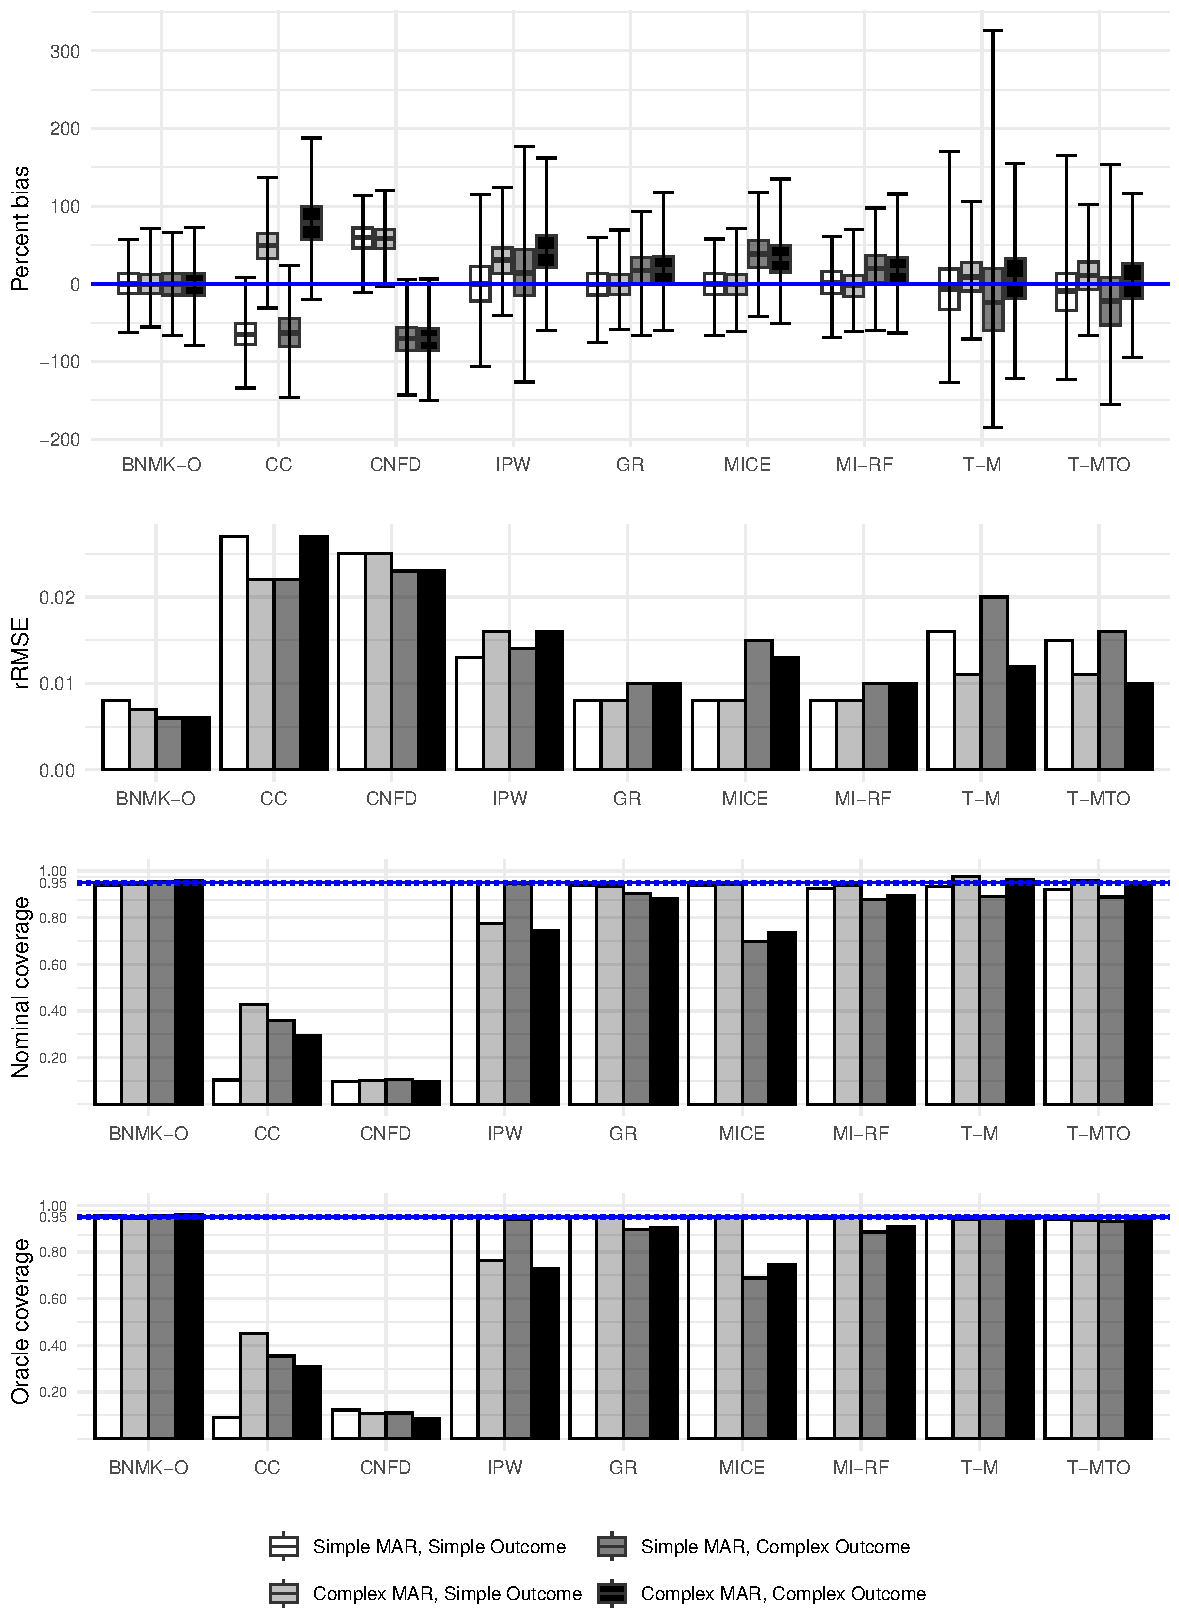
\includegraphics[width=0.75\textwidth,height=0.95\textheight]{./img/final4_mRD_oracle_truth_high_outcome_low_missing.pdf}
\end{frame}

\begin{frame} \frametitle{5\% outcome, 80\% missing data results: oracle mRD}
\centering
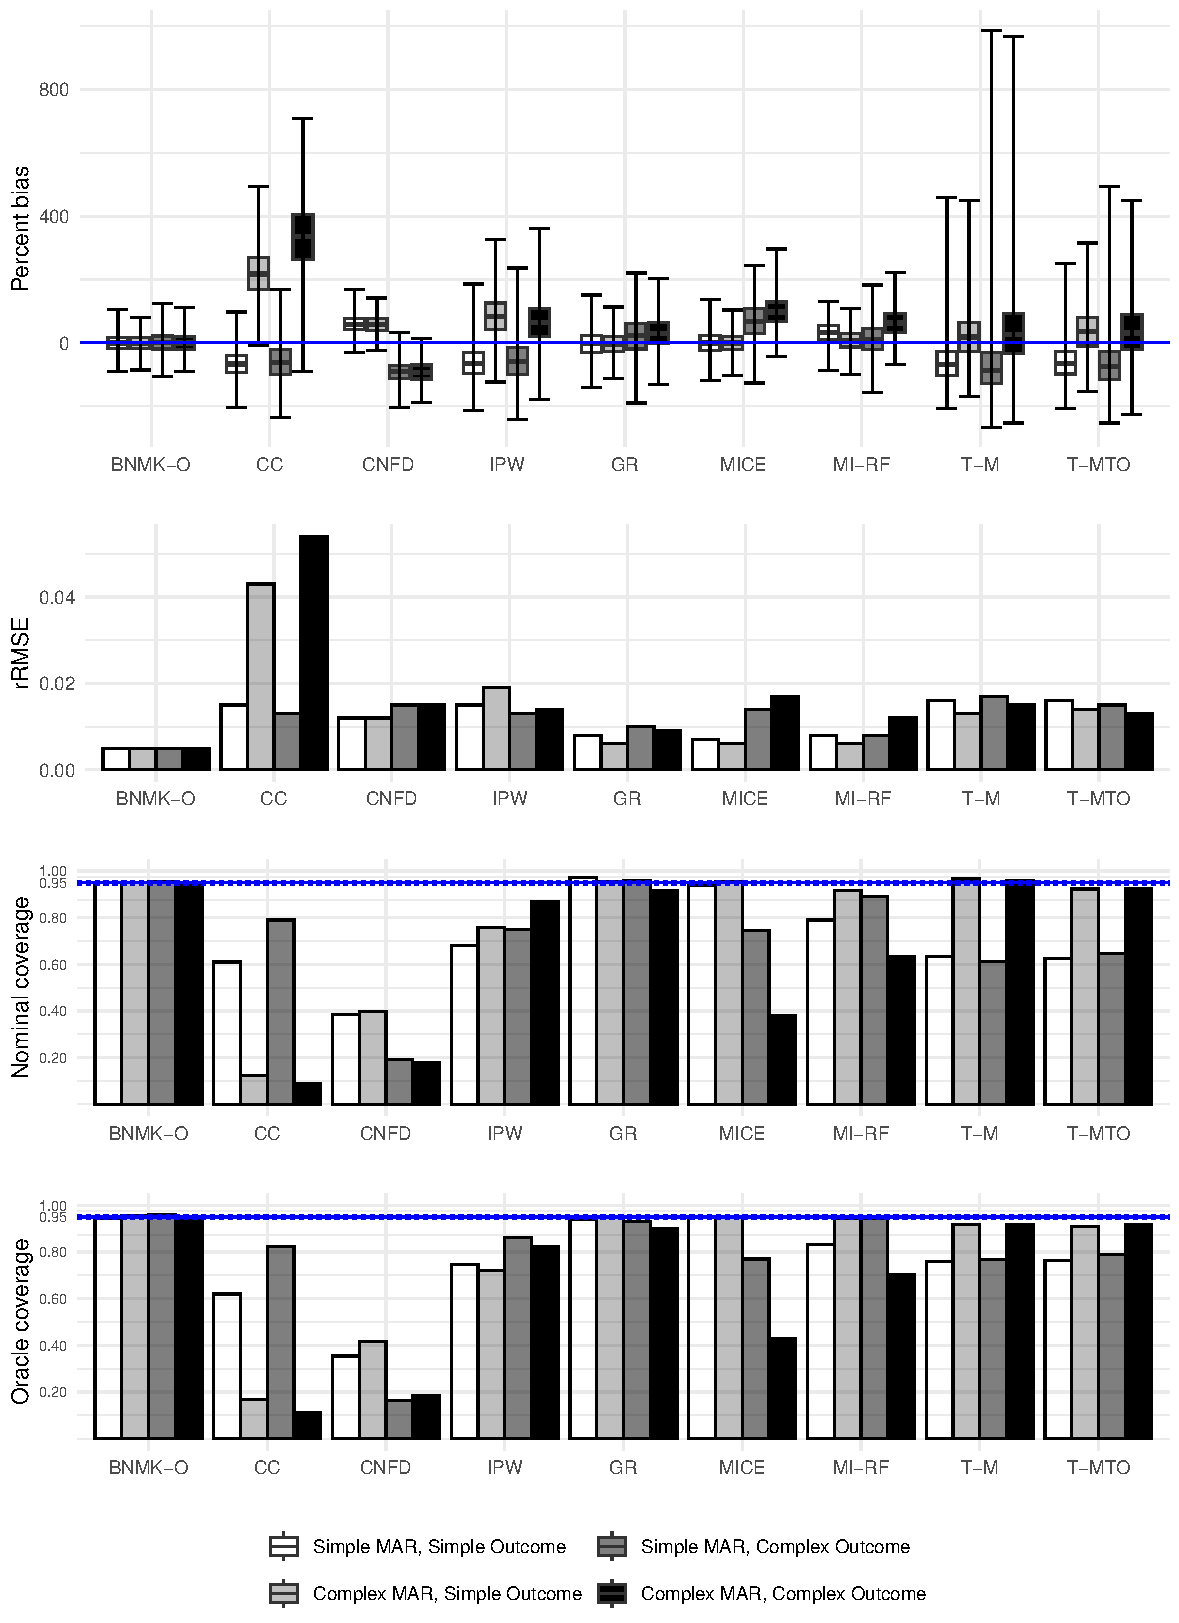
\includegraphics[width=0.75\textwidth,height=0.95\textheight]{./img/final4_mRD_oracle_truth_low_outcome_high_missing.pdf}
\end{frame}

% show base case, base case (80\%), rare-outcome 80\%

% \section{Plasmode simulations}
% \begin{frame} \frametitle{Plasmode data generation}
% Data-generating models:\vspace{-0.4cm}
% \begin{itemize}
%   \item $\pi$: tree or glm fit to entire cohort ($n = 112770$) to predict observation of PHQ-9
%   \item $g$: tree or glm fit to complete cohort ($n = 50337$) to predict assignment to psychotherapy vs antidepressant medication
%   \item $Q$: tree or glm fit to complete cohort
% \end{itemize}
% Other confounders: sex, age, Charlson comorbidity index, anxiety diagnosis in past year, self-harm in prior 6 months, psychiatric hospitalization in prior 5 years, alcohol use disorder in past year

% \end{frame}

% \begin{frame} \frametitle{Plasmode simulation results: oracle mRD}
% \centering
% 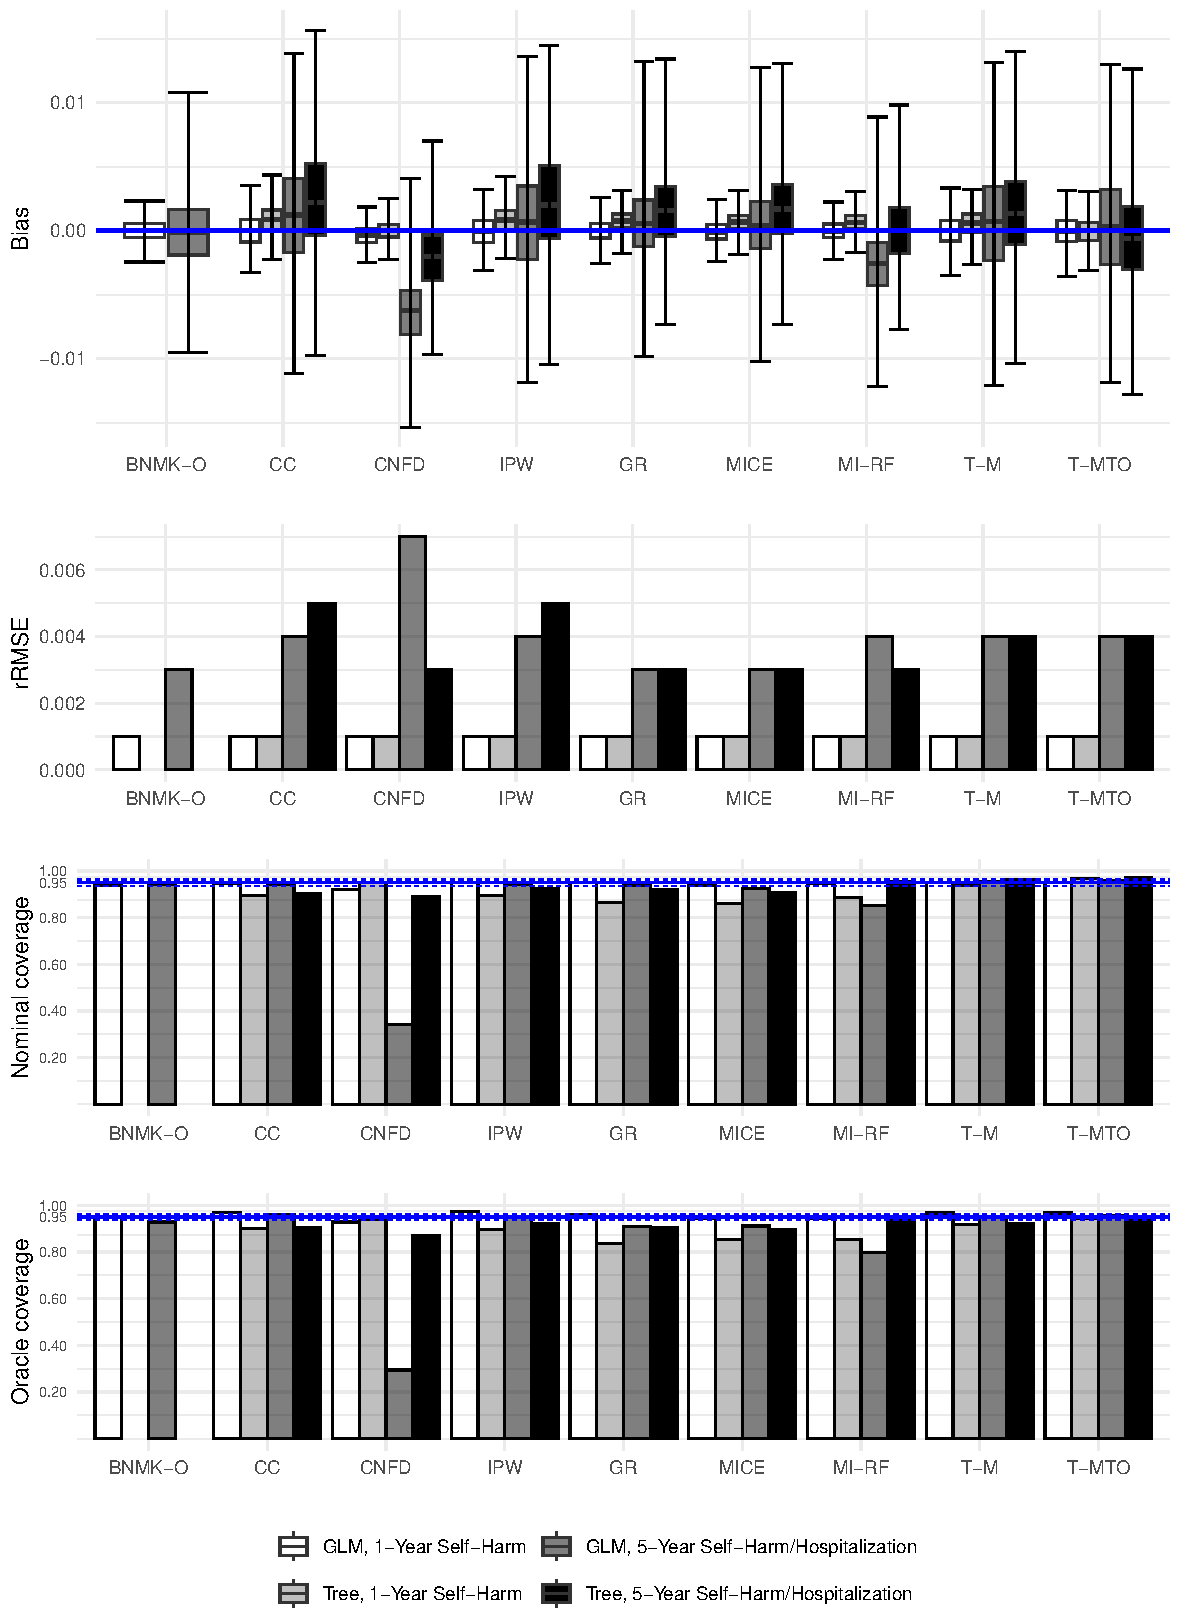
\includegraphics[width=0.75\textwidth,height=0.95\textheight]{./img/plasmode_final4_reg_bias_mRD_oracle_truth.pdf}
% \end{frame}

\section{Conclusion}

\begin{frame} \frametitle{Conclusions: part 1}

In our simulations, we observed:\vspace{-.4cm}
\begin{itemize}
  \item the importance of first choosing a target estimand, then an estimation procedure
  \item confounded and complete-case methods performed poorly
  \item at least one variant of MI often performed well, but no one variant performed well uniformly
  \item generalized raking among the best in the majority of settings
  \item TMLE often had small bias but larger variance
\end{itemize}
\begin{minipage}{0.45\textwidth}
For more, check out: \vspace{-.1cm}
\begin{itemize}
  \item the paper, \citet{williamson2026subsetcalibration}
  \item the repo, \url{https://github.com/PamelaShaw/Missing-Confounders-Methods}
\end{itemize}
\end{minipage}
\begin{minipage}{0.45\textwidth}
  \centering
  
\includegraphics[width=0.5\textwidth]{img/qr_code_arxiv_2412_15012.png}
\end{minipage}

\end{frame}

\begin{frame} \frametitle{Partial aside: better MI variances}
Common MI variance method: Rubin's rules \citep{little1987multiple} \vspace{-0.4cm}
\begin{itemize}
  \item Simple to apply!
  \item Invalid under uncongeniality (assumptions of the imputation model and analysis model are discordant)
\end{itemize}

The \citet{robins2000inference} estimator is robust to uncongeniality, but \vspace{-0.4cm}
\begin{itemize}
  \item has not been implemented in software
  \item has not been studied with chained equations (e.g., \texttt{mice})
  \item has not been studied with predictive mean matching (\texttt{mice} default)
\end{itemize}

\begin{minipage}{0.45\textwidth}
We have addressed these three gaps in recent work, with an R package that mimics the \texttt{mice} syntax to make RW variance easy!
\end{minipage}
\begin{minipage}{0.45\textwidth}
\centering
  
\includegraphics[width=0.5\textwidth]{img/arxiv_2610_12215_qr_rwpaper.png}
\end{minipage}

\end{frame}

\begin{frame} \frametitle{Acknowledgments: part 2}
\centering

\includegraphics[width=1\textwidth]{img/people_all.png}
\end{frame}

\begin{frame} \frametitle{Conditional generalized raking}
  Generalized raking for regression parameters $\beta$: \vspace{-0.4cm}
  \begin{enumerate}[<+->]
    \item Obtain an estimator $\pi_{IPW,n}$ of $\pi$ using logistic regression
    \item Estimate optimal raking variable $\eta_Q(v) = E\{\phi_\beta^F(Y,A,L) \mid V = v\}$
    \begin{itemize}
      \item $\phi_\beta^F$: ideal-data efficient influence function (EIF) vector for $\beta$ \citep{bickel1993efficient}
      \item EIF can be extracted from \texttt{glm} objects using \texttt{sandwich} package
      \item $\phi_\beta^F$ often estimated using multiple imputation \citep{oh2021improved}
    \end{itemize}
    \item Calibrate the weights: for a distance measure $d$, 
    \begin{align*}
      \pi_{n,CGR,i}^{-1} =& \ b_i^*\pi_{n,IPW,i}^{-1}, \text{ where } \label{eq:gr}\\
    b^* =& \ \min_{b \in \mathbb{R}^n}\sum_{i=1}^n R_i d(b_i\pi_{n,IPW,i}^{-1},\pi_{n,IPW,i}^{-1}) \\
    & \text{ subject to }  \sum_{i=1}^n \eta_{\beta,n}(V_i) = \sum_{i=1}^n R_i b_i \pi_{n,IPW,i}^{-1} \eta_{Q,n}(V_i).
    \end{align*}
    \item Obtain estimator $\beta_{n,GR}$ of $\beta$ by solving the estimating equation
    \begin{align*}
    \frac{1}{n}\sum_{i=1}^n\frac{R_i}{\pi_{n,CGR}(V_i)}S(Y_i, A_i,L_i;\beta) = 0.
\end{align*}
  \end{enumerate}
\end{frame}

\begin{frame} \frametitle{Conditional generalized raking}
  Recall: our goal is to estimate $\mu_1 = E\{E(Y \mid A = 1, L)\}$ (or another marginal parameter)
  
  First approach (taken in part 1): \textit{conditional} generalized raking \vspace{-0.2cm}
  \begin{itemize}
    \item Marginalize over the distribution of covariates
    \item Conditional because we first estimate $\beta$, then marginalize
  \end{itemize} \pause

  Define $Q_{n,CGR}(a,\ell) = h^{-1}\{(a,\ell)\beta_{n,GR}\}$. Then 
  \begin{align*}
    \mu_{1,n,CGR} :=& \ \frac{1}{n}\sum_{i=1}^n \frac{R_i}{\pi_{n,CGR}(V_i)} Q_{n,CGR}(1,L_i).
  \end{align*} \pause

  $\sqrt{n}(\mu_{1,n,CGR} - \mu_1) \to_d N(0, \sigma^2_{1,CGR})$, where $\sigma^2_{1,CGR} = \Omega\Sigma_\beta \Omega^\top$,
  \begin{align*}
    \Omega =& \ E\left\{\frac{R}{\pi(V)}\nabla h^{-1}(1,1,L;\beta)\right\}, \text{ and } \\
    \Sigma_\beta =& \ E\{\phi_\beta(Y,A,L) \phi_\beta(Y,A,L)^\top\}.
  \end{align*}
\end{frame}

\begin{frame} \frametitle{Conditional generalized raking}
  Advantages: \vspace{-0.4cm} 
  \begin{itemize}
    \item Inherits theory from GR estimator of regression parameters
    \item Doubly-robust for missing data: consistent if $\pi$ or $\eta_Q$ are consistent
    \item Estimation built on standard software (e.g., \texttt{survey})
  \end{itemize} \pause

  Drawbacks:\vspace{-0.4cm}
  \begin{itemize}
    \item Point estimation requires estimating $\beta$, not of primary interest
    \item Variance relies on delta method
  \end{itemize}
\end{frame}

\begin{frame} \frametitle{Efficient influence functions}
  Idea: rake directly on the EIF for the marginal parameter!

  In parametric models with complete data, EIF for regression coefficient vector $\beta$, $\phi_\beta^F$, is a function of the Fisher information and the score. \pause

  In nonparametric model with complete data, EIF for treatment-specific means well-known:
  \begin{align*}
    \phi_{\mu_1,NP}^F(y,a,\ell) =& \ \frac{I(a = 1)}{g(\ell)}\{y - Q(a,\ell)\} + Q(1,\ell) - E\{Q(1,L)\}.
  \end{align*} \pause

  With some work, we can obtain the EIF for the treatment-specific mean in a parametric model \citep{tsiatis2006semiparametric}:
  \begin{align*}
    \phi_{1,P}^F(y,a,\ell) := E\{\phi_{\mu_1,NP}(Y,A,L)S^\top_\beta(Y,A,L)\}I_\beta^{-1}S_\beta(y,a,\ell),
  \end{align*} 
  where $I$ is the information and $S$ is the score. 

  EIF in observed-data model (where some data are missing) is a transformation of this EIF.
\end{frame}

\begin{frame} \frametitle{Marginal generalized raking}
  Goal: estimate $\mu_1$ directly

  Approach: \textit{marginal} generalized raking \vspace{-0.2cm}
  \begin{enumerate}[<+->]
    \item Obtain an estimator $\pi_{IPW,n}$ of $\pi$ using logistic regression
    \item Estimate optimal raking variable $\eta(v) = E\{\phi_{1,P}^F(Y,A,L) \mid V = v\}$
    \begin{itemize}
      \item $\phi_{1,P}^F$: ideal-data EIF of $\mu_1$
      \item Estimate $\eta$ using, eg, MI
    \end{itemize}
    \item Calibrate the weights: for a distance measure $d$, 
    \begin{align*}
      \pi_{n,GR,i}^{-1} =& \ b_i^*\pi_{n,IPW,i}^{-1}, \text{ where } \\
    b =& \ \min_{b \in \mathbb{R}^n}\sum_{i=1}^n R_i d(b_i\pi_{n,IPW,i}^{-1},\pi_{n,IPW,i}^{-1}) \\
    & \text{ subject to }  \sum_{i=1}^n \eta_{n}(V_i) = \sum_{i=1}^n R_i b_i \pi_{n,IPW,i}^{-1} \eta_{n}(V_i).
    \end{align*}
    \item Obtain estimator $\mu_{1,n,MGR}$ of $\mu_1$:
    \begin{align*}
    \mu_{1,n,MGR} :=& \ \frac{1}{n}\sum_{i=1}^n \frac{R_i}{\pi_{n,GR}(V_i)}\left[\frac{I(A_i = 1)}{g_n(L_i)}\{Y_i - Q_n(1,L_i)\} + Q_n(1,L_i)\right].
\end{align*}
  \end{enumerate}
\end{frame}

\begin{frame} \frametitle{Marginal generalized raking}
  Marginal generalized raking is asymptotically equivalent to the augmented IPW estimator \citep{robins1994estimation},
  \begin{align*}
    \mu_{1,n,AIPW} :=& \ \frac{1}{n}\sum_{i=1}^n \left(\frac{R_i}{\pi_{n,IPW}(V_i)}\left[\frac{I(A_i = 1)}{g_n(L_i)}\{Y_i - Q_n(1,L_i)\} + Q_n(1,L_i)\right] \right.\\
    & \ \ \ \ \ \ \ \ \ \ \  + \left. \frac{\{\pi_{n,IPW} - R_i\}}{\pi_{n,IPW}}\eta_n(V_i)\right).
  \end{align*} 

  Under some regularity conditions, $\sqrt{n}(\mu_{1,n,MGR} - \mu_1) \to_d N(0, \sigma^2)$, with variance $\sigma^2$ based on the observed-data EIF.

  $\mu_1$ is also \textit{multiply robust}: consistent if (i) $Q$ or $g$ and (ii) $\pi$ or $\eta$ are estimated sufficiently well.
\end{frame}

\begin{frame} \frametitle{Numerical experiments}
  All fully-synthetic data with missing data in the confounders:\vspace{-0.4cm}
  \begin{itemize}
    \item Scenarios 1a (continuous) \& 1b (binary): correctly-specified models, 20\% missing data probability.
    \item Scenarios 2a \& b: rarer binary outcome (10\%), more missing data (50\%).
    \item Scenarios 3a \& b: S2 with misspecified propensity score model $g$ (missing confounder).
    \item Scenarios 4a \& b: S2 with misspecified outcome regression model $Q$ (missing confounder).
    \item Scenarios 5a \& b: S2 with misspecified missing data model $\pi$.
  \end{itemize} 

  Estimators: CGR (with IPTW and regression adjustment), MGR, AIPCW-AIPTW.
\end{frame}

\begin{frame} \frametitle{Results: Scenario 2b (correctly-specified models)}
  \centering
  \hspace*{-1cm}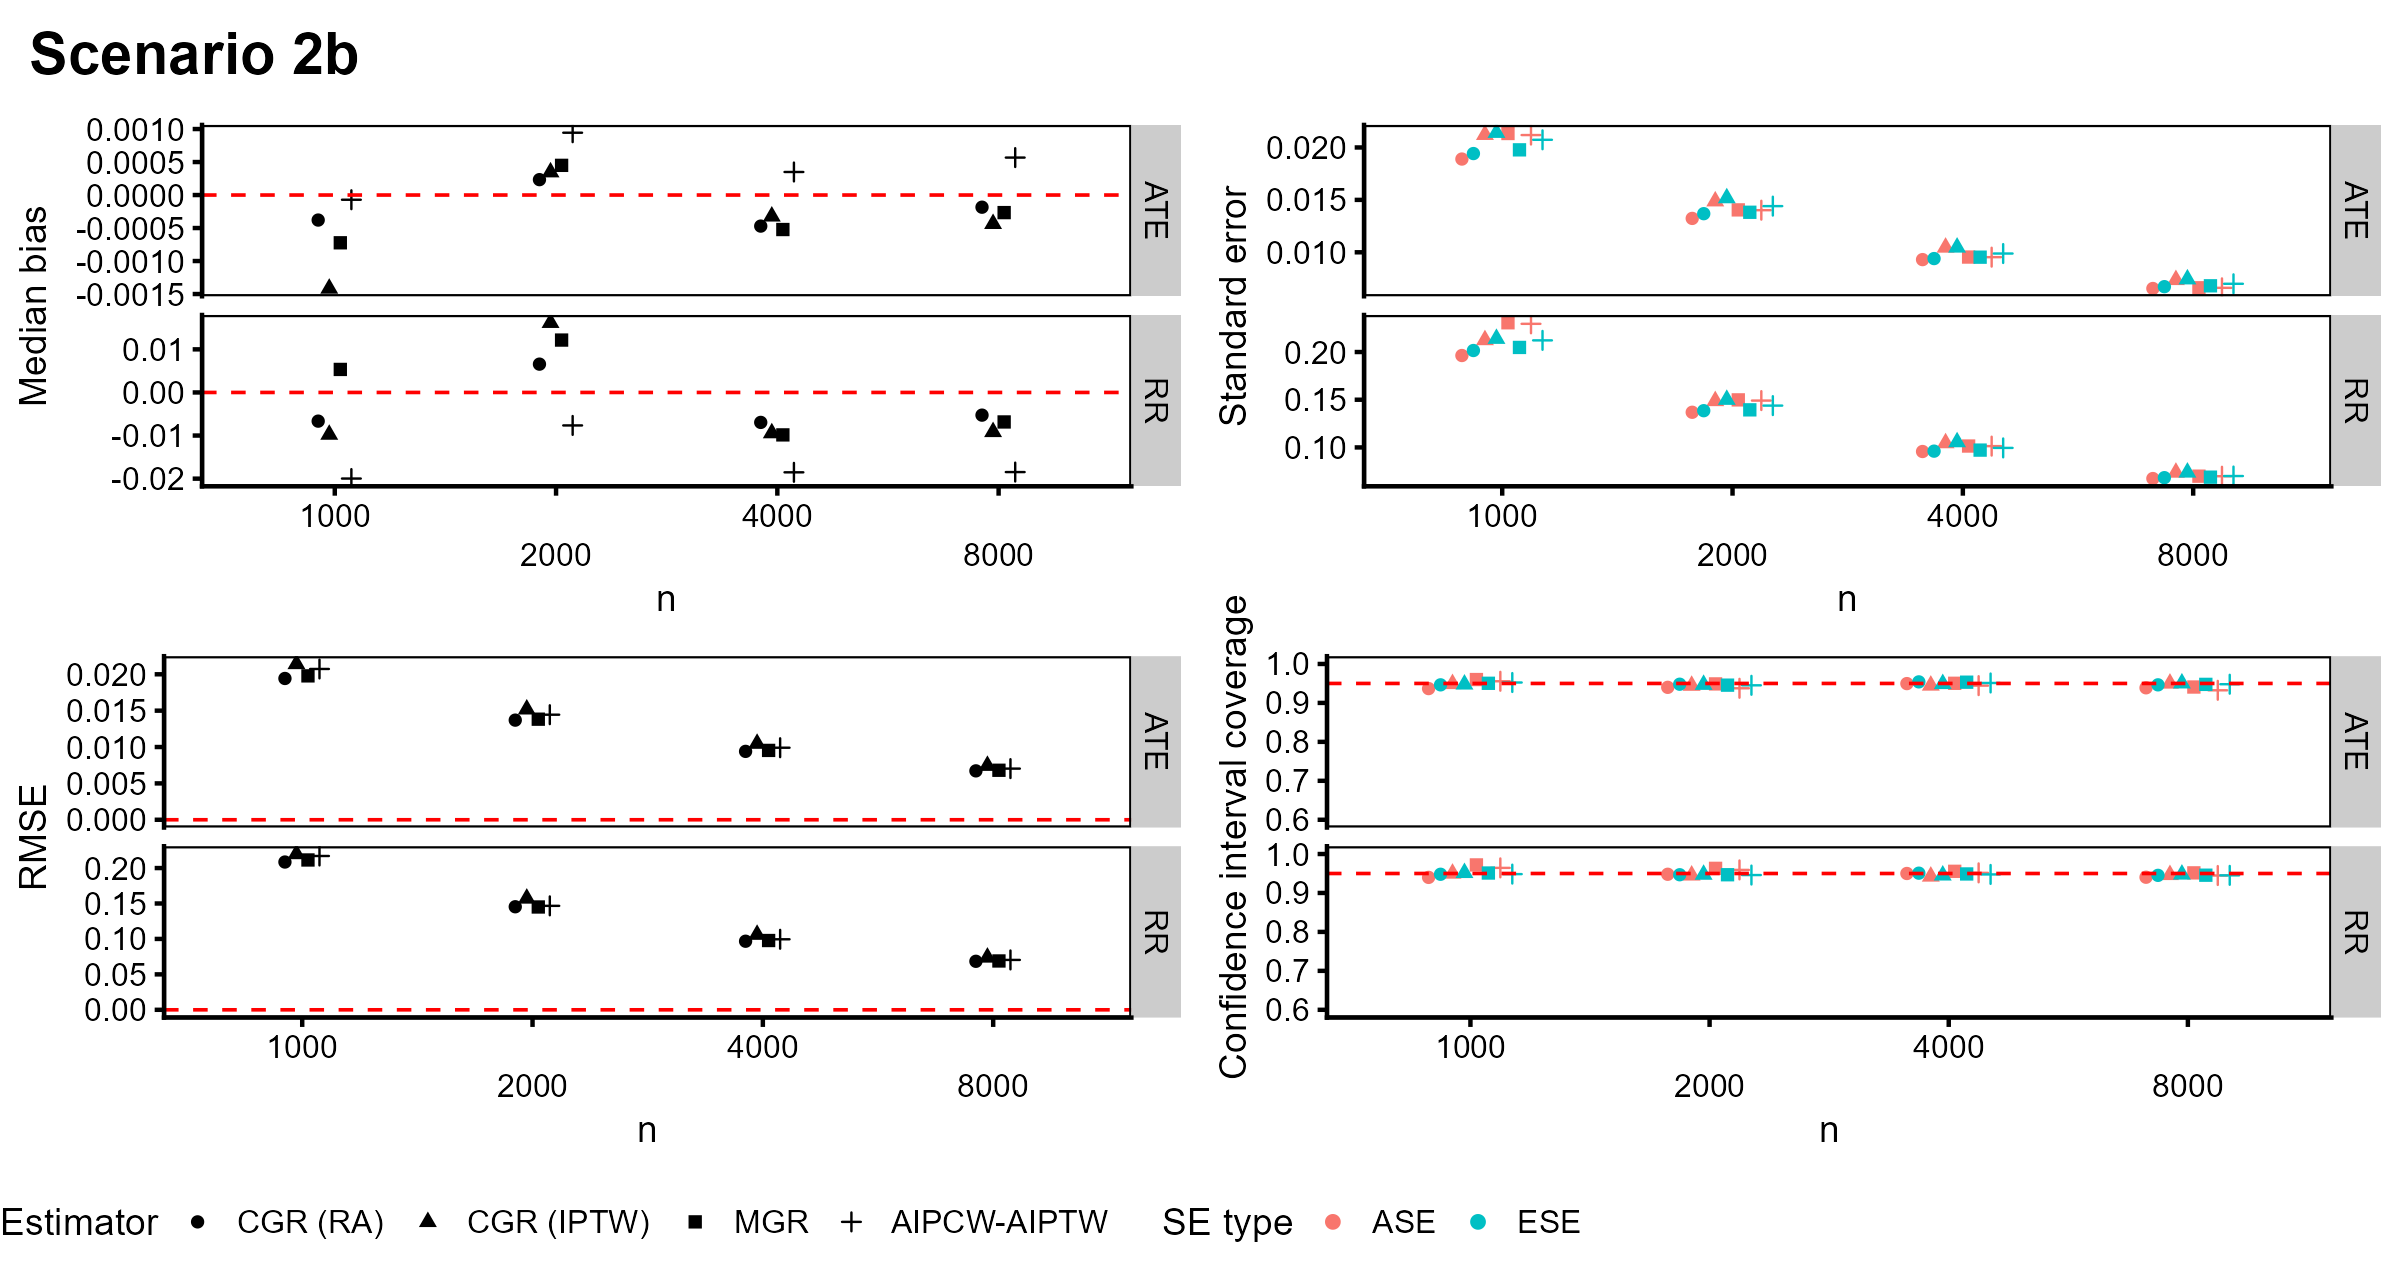
\includegraphics[width=1.2\textwidth]{img/sim_combined_performance_plot_s4.png}
\end{frame}

\begin{frame} \frametitle{Results: Scenario 3b (misspecified $g$)}
  \centering
  \hspace*{-1cm}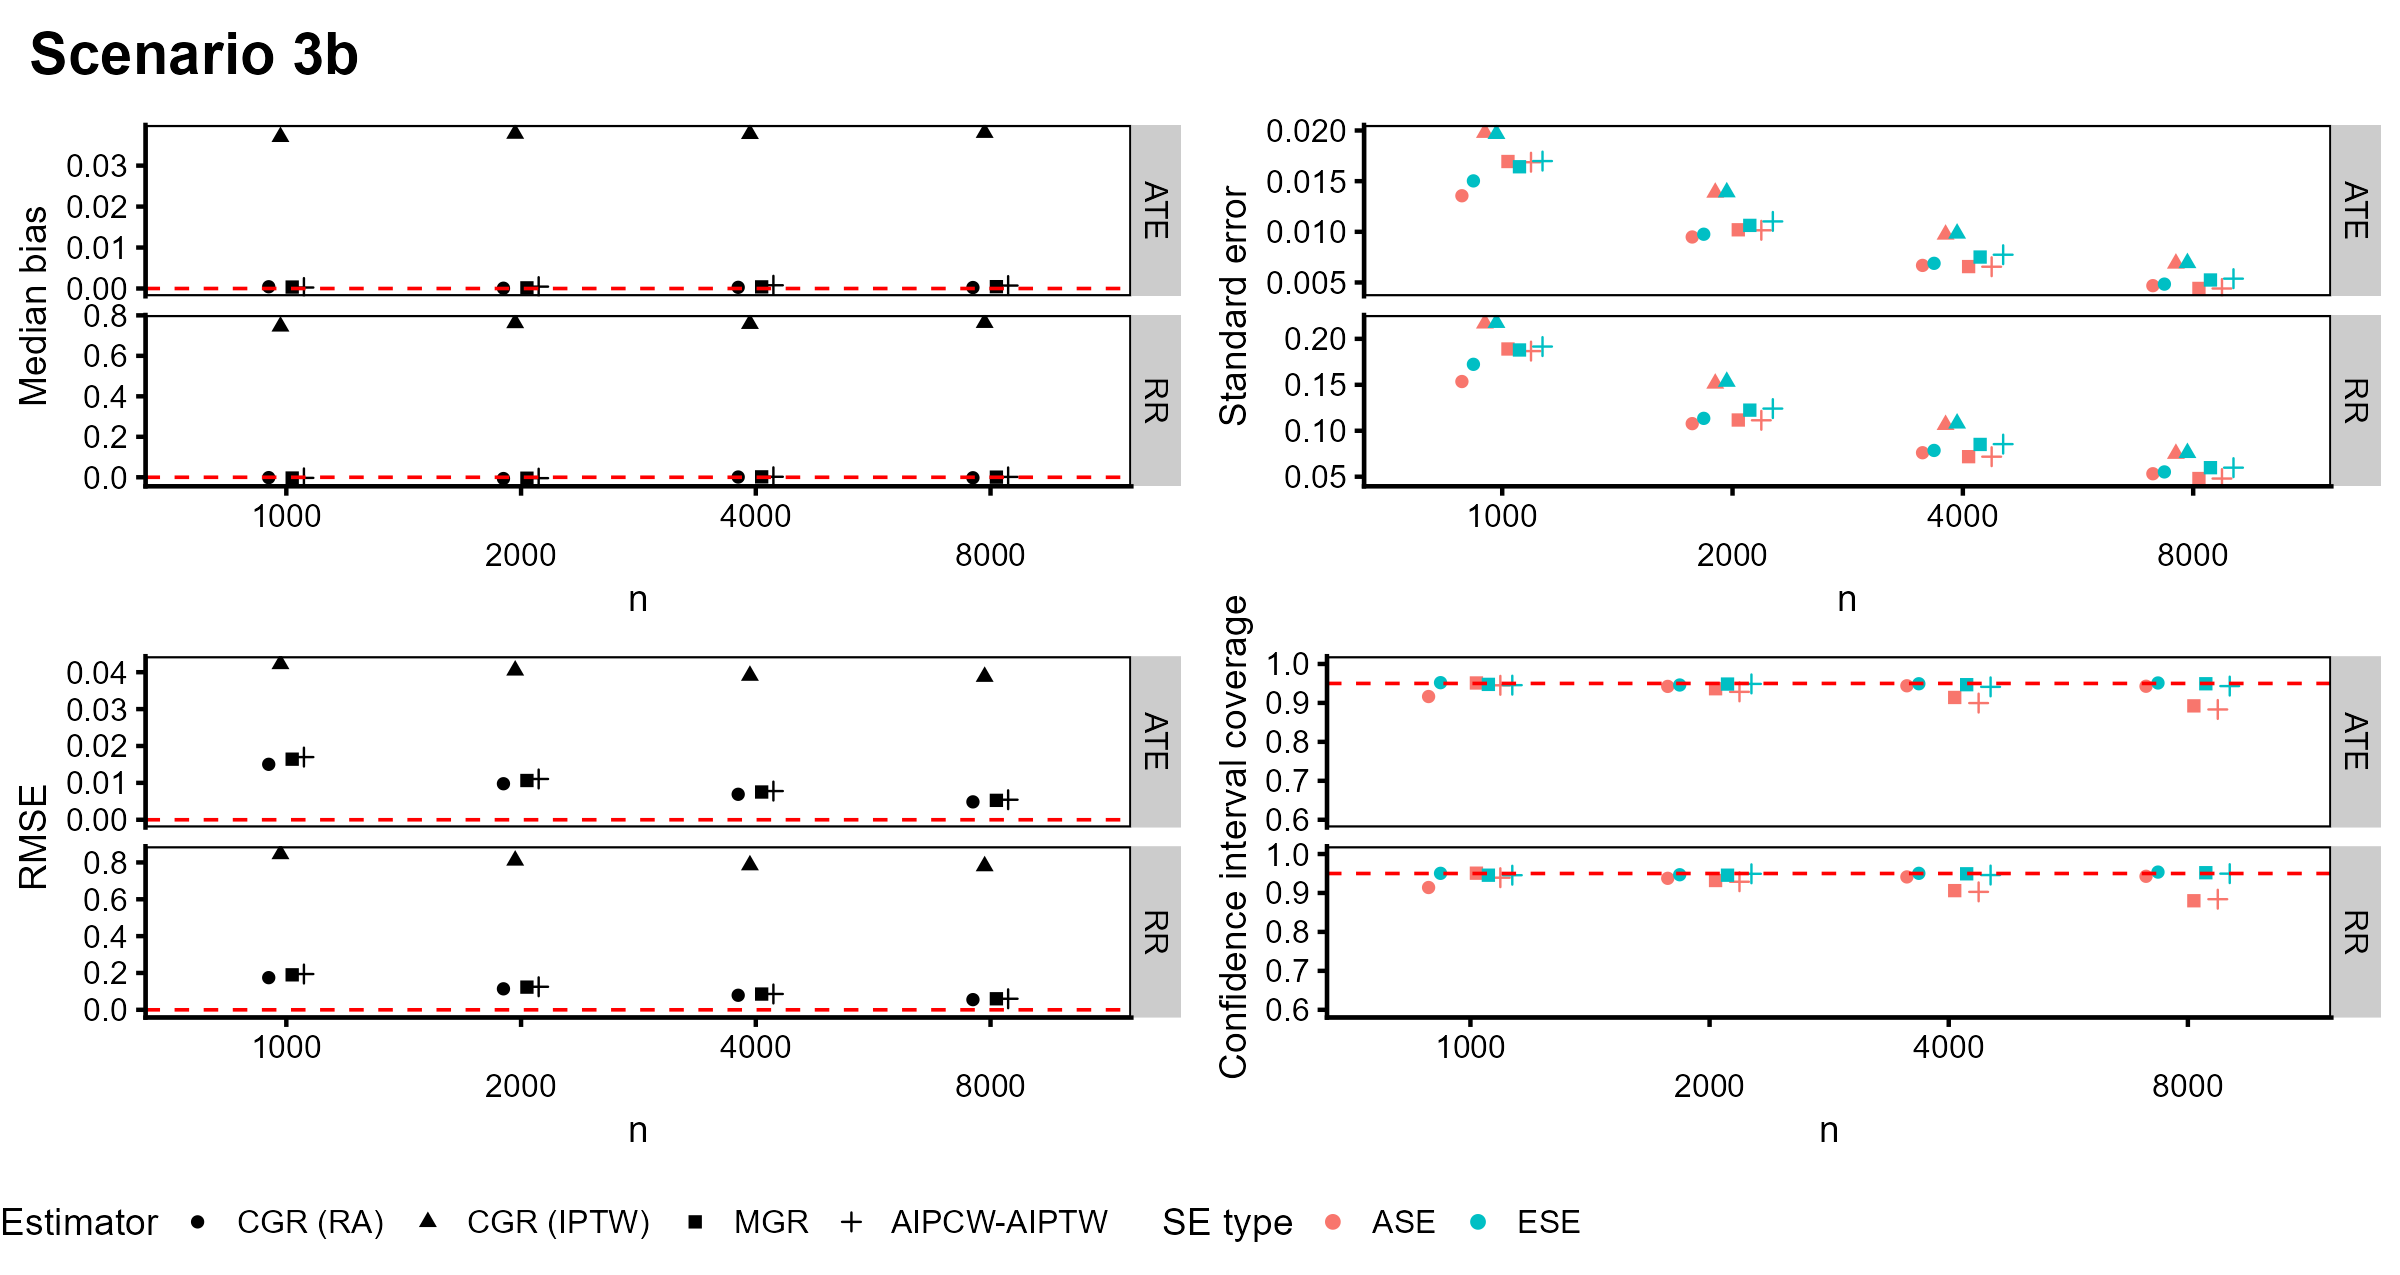
\includegraphics[width=1.2\textwidth]{img/sim_combined_performance_plot_s6.png}
\end{frame}

\begin{frame} \frametitle{Results: Scenario 4b (misspecified $Q$)}
  \centering
  \hspace*{-1cm}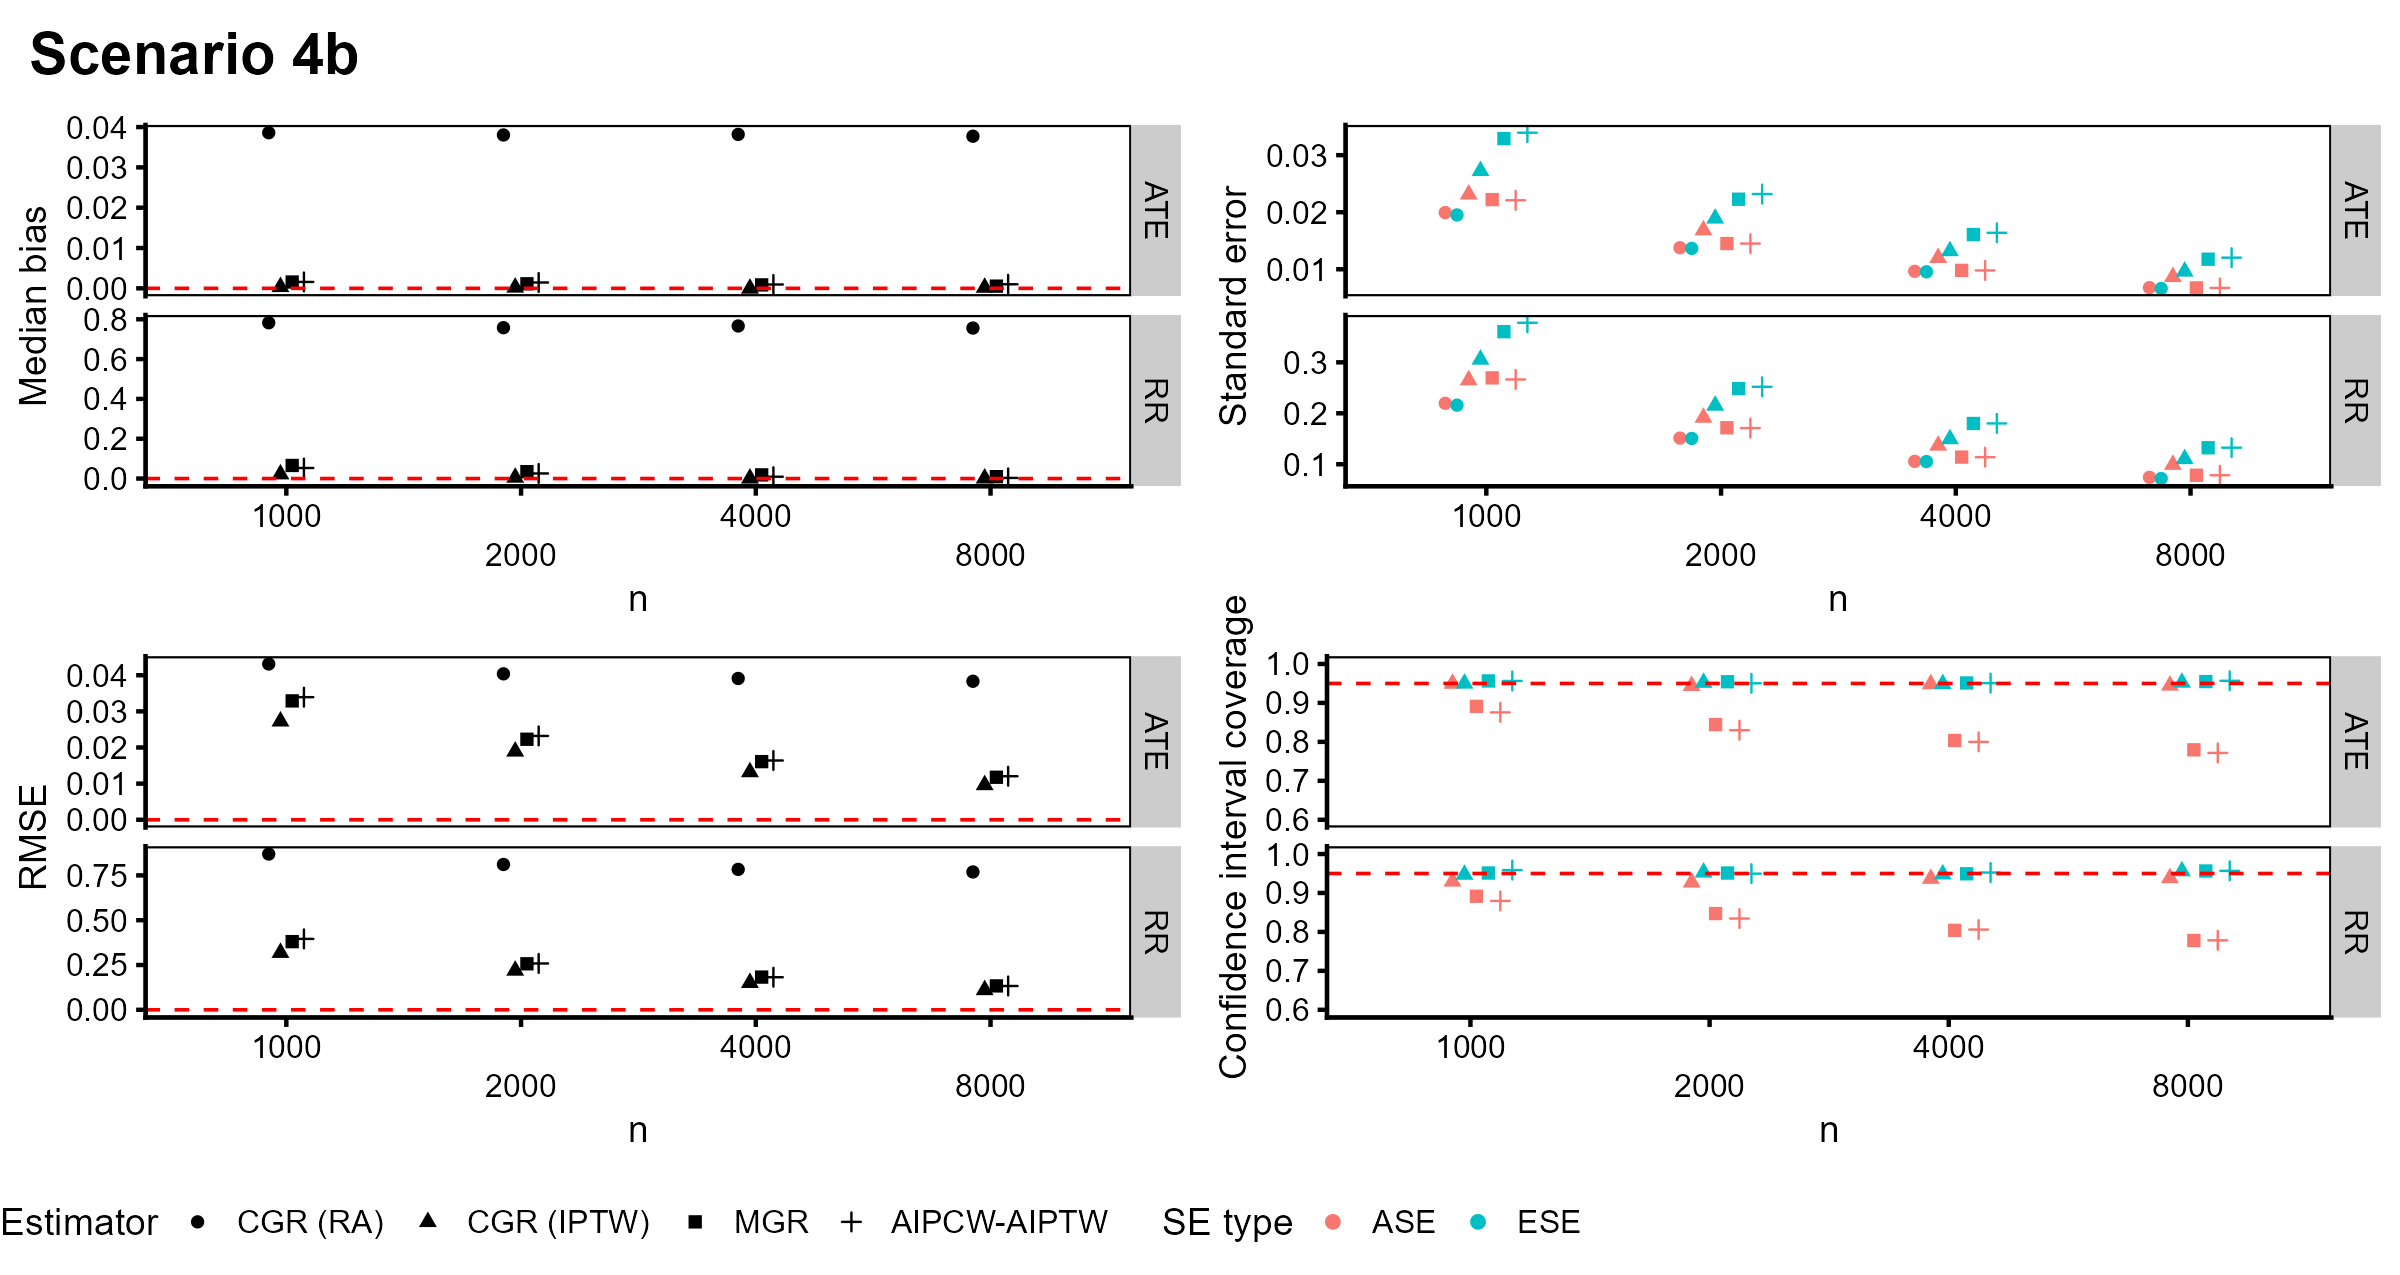
\includegraphics[width=1.2\textwidth]{img/sim_combined_performance_plot_s8.png}
\end{frame}

\begin{frame} \frametitle{Results: Scenario 5b (misspecified $\pi$)}
  \centering
  \hspace*{-1cm}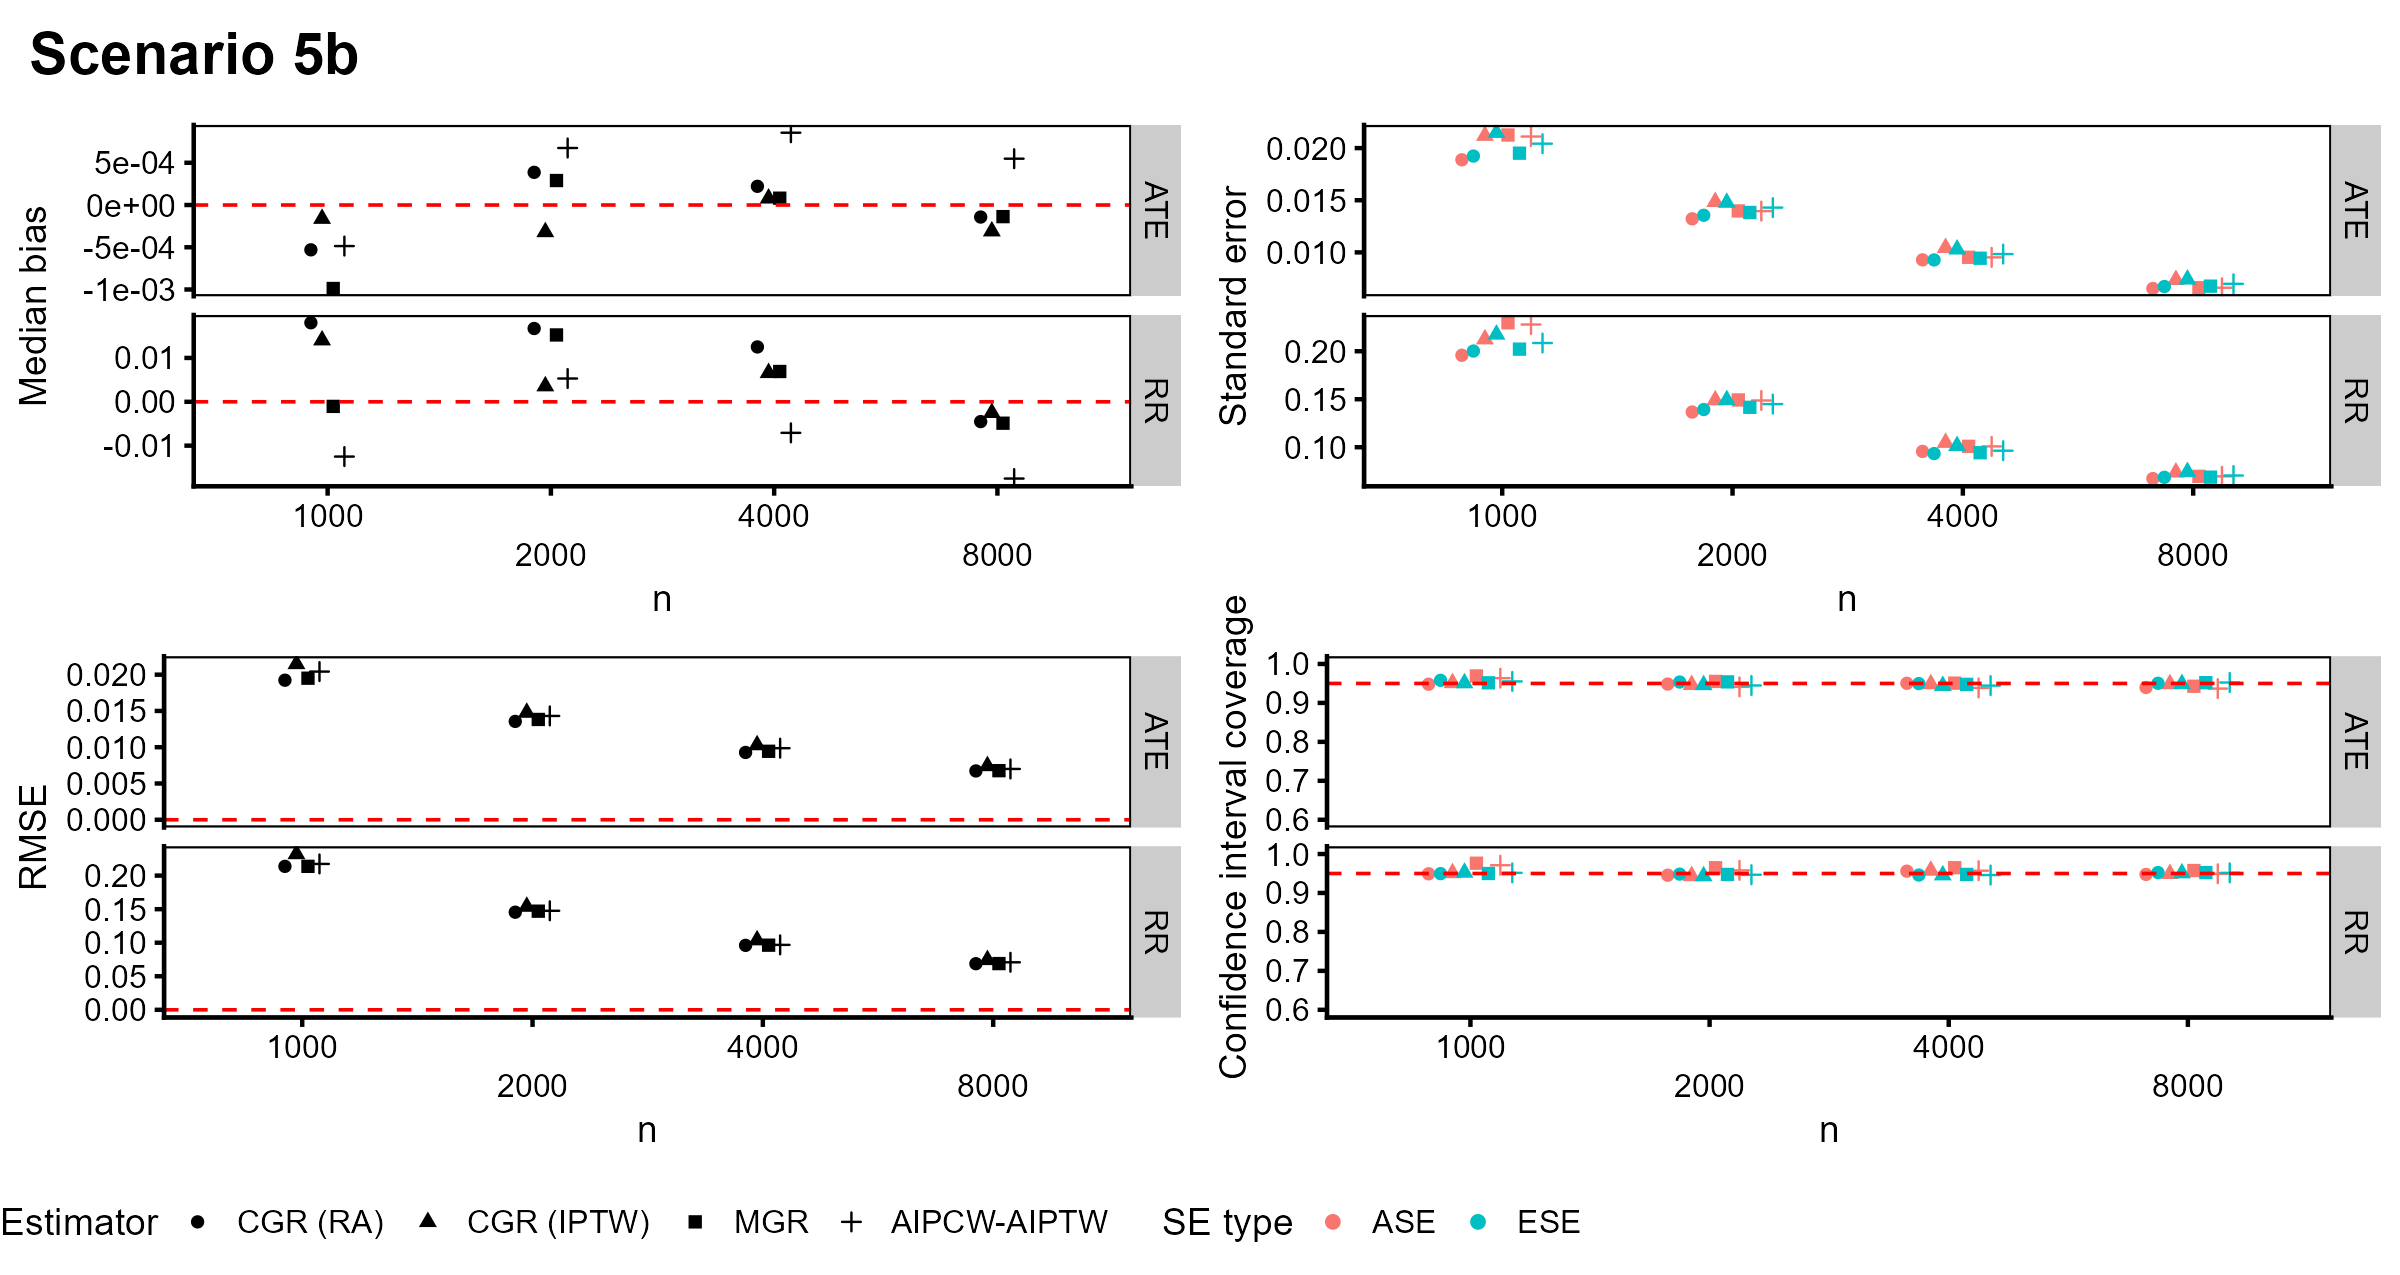
\includegraphics[width=1.2\textwidth]{img/sim_combined_performance_plot_s10.png}
\end{frame}

\begin{frame} \frametitle{Conclusions: part 2}

  Marginal generalized raking is: \vspace{-0.4cm}
  \begin{itemize}
    \item equivalent to AIPW for marginal parameters -- extends result for regression parameters
    \item a more convenient method for calculating AIPW estimators, through R implementation in \texttt{survey}
    \item more efficient than CGR, particularly with non-identity link functions
  \end{itemize}

  In current work, we are extending to ML estimators and showing asymptotic equivalence with TMLE.

  \begin{minipage}{0.5\textwidth}
    \faGithub \url{https://github.com/bdwilliamson }\\
    \faGlobe \url{https://bdwilliamson.github.io}\\
    \faEnvelope \texttt{brian.d.williamson@kp.org}
  \end{minipage}
  \begin{minipage}{0.45\textwidth}
    \centering
    
\includegraphics[width=0.5\textwidth]{img/qr_arxiv_2607_29629.png}
    
    Manuscript on arXiv!
  \end{minipage}
  
\end{frame}

\begin{frame}[allowframebreaks] \frametitle{References}
  \nocite{*}
  \bibliographystyle{chicago}
  \bibliography{pubs}

\end{frame}

  
\end{document}
  